\chapter{Mixed-Bag Solver Overview}\label{chap:mixedBagSolver}

This thesis' Mixed-Bag Solver supports Type~1, Type~2, and Mixed-Bag puzzles.  It consists of five distinct stages, namely: segmentation, stitching, hierarchical clustering of segments, seed piece selection, and final assembly.  The flow of the algorithm is shown in Figure~\ref{fig:multipuzzleSolverArchitecture}; the pseudocode for the solver, including the input(s) and output of each stage is shown in Algorithm~\ref{alg:mixedBagSolver}.

The following subsections describe each of Mixed-Bag Solver's stages/subfunctions.  It also discusses the assembler (not shown in Figure~\ref{fig:multipuzzleSolverArchitecture}), which is a separate but associated component of the architecture.

\begin{figure}[ht!]
	\centering
		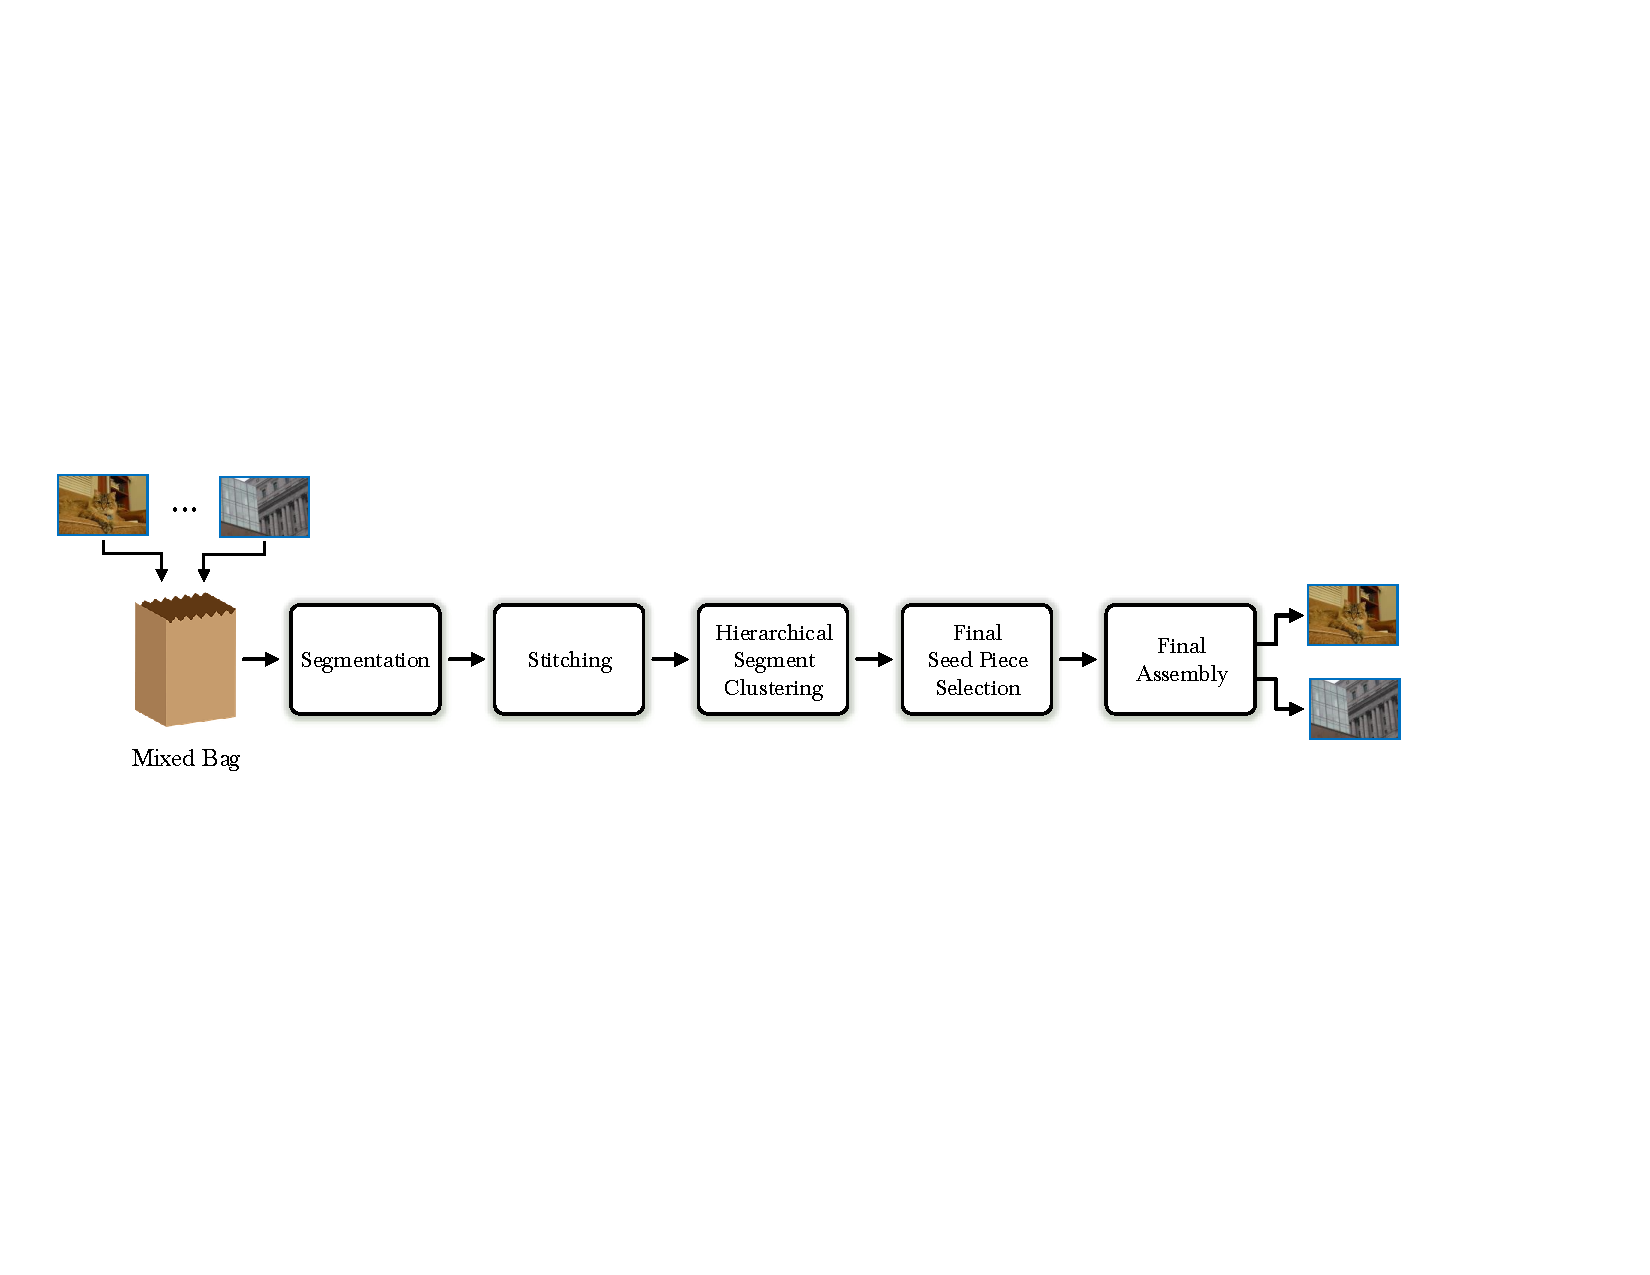
\includegraphics[width=1.0\textwidth]{images/cropped_algorithm_structure_overview.pdf}
	\caption{Components of the Mixed-Bag Puzzle Solver}\label{fig:multipuzzleSolverArchitecture}
\end{figure}

\begin{algorithm}[tb]
\caption{Pseudocode for the Mixed Bag Solver}\label{alg:mixedBagSolver}
\begin{algorithmic}[1]
\Function{MixedBagSolver}{$all\_pieces$}
    \State $solved\_segments \gets \textproc{Segmentation}\text{(} all\_pieces \text{)}$
	\State $overlap\_matrix \gets \textproc{Stitching}\text{(} solved\_segments \text{, } all\_pieces \text{)}$
	\State $clusters \gets \textproc{HierarchicalClustering} \text{(}solved\_segments \text{, } overlap\_matrix \text{)}$
	\State $puzzle\_start\_pieces \gets \textproc{FindStartingPieces} \text{(} clusters \text{)}$
	\State $solved\_puzzles \gets \textproc{RunFinalAssembly} \text{(} puzzle\_start\_pieces \text{, } all\_pieces \text{)}$
    \State \Return $solved\_puzzles$
\EndFunction
\end{algorithmic}
\end{algorithm}

\section{Assembler}\label{sec:SolverAssembler}

The assembler assigns the placement (and optionally rotation) of the puzzle pieces in the solved puzzle.  The Mixed-Bag Solver's architecture is largely independent of the particular assembler used.  Hence, any improvements or modifications to the assembler can be directly incorporated into the Mixed-Bag Solver to improve the solver's performance.  What is more, if a particular assembler performs better than others for a particular application, the assemblers can be interchanged.  This provides the Mixed-Bag Solver with significant flexibility and upgradability to maximize performance across a wide range of applications.

For all experiments in this thesis, the assembler proposed proposed by Paikin~\& Tal~\cite{paikin2015}.  As mentioned in Chapter~\ref{chap:previousWork}, their assembler is the current state of the art and is one of the few algorithms that natively supports Mixed-Bag puzzles.

\subsection{Assembler Time Complexity}


\subsection{Assembler Implementation}\label{sec:assemblerImplementation}

As of this publication, the implementation of Paikin~\&~Tal's algorithm is not open-source.  Hence, their algorithm was implemented as part of this thesis based off of the description in~\cite{paikin2015}.  This thesis' implementation is in the Python programming language and is fully open-source.

\section{Segmentation}\label{sec:Segmentation}

As detailed in Algorithm~\ref{alg:mixedBagSolver}, segmentation stages takes as input only the bag of puzzle pieces created from the original images; unlike all other solvers to date, this algorithm takes no other inputs.  The role of segmentation is to a basic provide structure to the unordered input.  This is done by partitioning the pieces into disjoint sets, referred to here as segments.  These segments are groups of puzzle pieces where there is a high degree of confidence that the pieces are assembled correctly.

Algorithm~\ref{alg:segmentation} outlines the basic segmentation framework; the implementation is iterative and will have one or more rounds.  In each round, all pieces not yet assigned to a saved segment are assembled as if they all belong to a single ground-truth image.  This eliminates the need to make any assumptions regarding the input at this early stage of the solver.  It is expected that pieces from the same input puzzle may be assigned to multiple separate segments.  Section~\ref{} describes how these multiple segments are merged using hierarchical clustering.

After the single puzzle is assembled in each round, the solved puzzle is then divided into segments; the procedure for this is described in Section~\ref{sec:segmentPuzzle}.  Assuming the largest segment exceeds the minimum allowed size\footnote{For this thesis, it was observed that a minimum segment size of 7 provided the best balance between solution quality and algorithm execution time.}, it is passed to the next stage of the Mixed-Bag Solver.  

The term ``\textit{$\alpha$}'' in Algorithm~\ref{alg:segmentation} defines which segments in a given segmentation round are passed to the next stage of the Mixed-Bag Solver.  In this thesis, \textit{$\alpha$} was set to 0.5, meaning any segment that was at least half the size of the largest segment in that round (and larger than the minimum segment size) is saved.  This scalar value provides sufficient balance between ensuring the largest segments for analysis with limiting the execution time of this stage.

Once a piece is assigned to a saved segment, it is removed from the set of unassigned pieces.  Hence, those pieces will not be placed in the next segmentation round.  Segmentation continues until all pieces have been assigned to sufficiently large segments, or no segment exceeds the minimum allowed segment size.

\begin{algorithm}[tb]
\caption{Pseudocode for the Segmentation Algorithm}\label{alg:segmentation}
\begin{algorithmic}[1]
\Function{Segmentation}{$all\_pieces$}
    \State $\textit{saved\_segments} \gets \{ \}$
    \State $unassigned\_pieces \gets \{ \textit{all\_pieces} \}$
    \Loop
        \State $solved\_puzzle \gets \textproc{RunSinglePuzzleAssembly}(unassigned\_pieces)$
        \State $puzzle\_segments \gets \textproc{SegmentPuzzle}(solved\_puzzle\text)$
\item[]
        \State $max\_segment\_size \gets \text{maximum size of segment in } solved\_segments$
        \If{$max\_segment\_size \text{ < } smallest\_allowed$}
			\State \Return $saved\_segments$
        \EndIf
\item[]
        \ForEach{$segment \in puzzle\_segments$}
            \If{$|segment| \text{ > } \alpha \times max\_segment\_size$}
                \State $\text{add } segment \text{ to } saved\_segments$
                \State $\text{remove pieces in } segment \text{ from } unassigned\_pieces$
            \EndIf
        \EndFor
	\EndLoop
\EndFunction
\end{algorithmic}
\end{algorithm}

\subsection{The \textproc{SegmentPuzzle} Function}\label{sec:segmentPuzzle}

The \texttt{SegmentPuzzle} function shown in Algorithm~\ref{alg:segmentPuzzle} is adapted from the kernel growing segmentation procedure proposed by Pomeranz \textit{et al.}, where it was shown to have greater than 99.7\% accuracy identifying genuine neighbors \cite{pomeranz2011}. The kernel of each segment is a single seed piece.

\begin{algorithm}[tb]
\caption{Pseudocode to Segment a Solved Puzzle}\label{alg:segmentPuzzle}
\begin{algorithmic}[1]
\Function{SegmentPuzzle}{$solved\_puzzle$}
    \State $puzzle\_segments \gets \{ \}$
    \State $unassigned\_pieces \gets \{ \text{all pieces in } solved\_puzzle \}$
\item[]
    \While{$|unassigned\_pieces| \text{ > } 0$}
        \State $segment \gets \text{ new empty segment}$
        \State $seed\_piece \gets \text{next piece in } unassigned\_pieces$
        \State $queue \gets [seed\_piece]$
\item[]
        \While{$|queue| \text{ > } 0$}
            \State $piece \gets \text{next piece in } queue$
            \State $\text{add } piece \text{ to } segment$
\item[]
            \ForEach{$neighbor\_piece \text{ of } piece$}
            	\If{$\textproc{IsBestBuddies}(neighbor\_piece, piece)$}
            		\State $\text{add } neighbor\_piece \text{ to } \textit{queue}$
            		\State $\text{remove } neighbor\_piece \text{ from } unassigned\_pieces$
            	\EndIf
            \EndFor
        \EndWhile
\item[]
        \State $\textit{articulation\_points} \gets \textproc{FindArticulationPoints}(\textit{segment})$
        \State $\text{remove } \textit{articulation\_points} \text{ from } \textit{segment}$
\item[]
		\State $\textit{disconnected\_pieces} \gets \textproc{FindDisconnectedPieces}(\textit{segment},\textit{seed\_piece})$ 
		\State $\text{remove } \textit{disconnected\_points} \text{ from } \textit{segment}$
\item[]
        \State $\text{add } \textit{articulation\_points} \text{ and } \textit{disconnected\_pieces} \text{ to } \textit{unassigned\_pieces}$               	
		\State $\text{add } segment \text{ to } puzzle\_segments$	
    \EndWhile
\item[]
    \State \Return $\textit{puzzle\_segments}$
\EndFunction
\end{algorithmic}
\end{algorithm}

Whenever a piece is added to a segment, the algorithm examines all of the piece's neighbors.  Any of the adjacent pieces that satisfy the ``best buddy'' criteria as defined in Chapter~\ref{chap:previousWork} are also added to the segment.  This process continues until the segment has no neighboring best buddies. In Pomeranz \textit{et al.}'s algorithm, no changes were made to the segment after it reached the maximum size.  This approach can be sufficient when solving only a single puzzle at a time as they did.  However, it is common in Mixed-Bag puzzles that two or more correctly assembled segments are joined into a single cluster by very linking, usually in the form of narrow bridges no wider than a single piece.  These tenuous links are broken to prevent erroneous segment merging.  

\subsection{Articulation Points}\label{sec:ArticulationPoints}

A segment can be modeled as a graph with a single connected component.  The individual puzzle pieces represent the vertices while the edges are the interpiece best buddy relationships as defined in Chapter~\ref{chap:previousWork} and determined in Algorithm~\ref{} by the function ``$\textproc{IsBestBuddies}$''.  An articulation point is any vertex (i.e., puzzle piece) whose removal increases the number of connected components.  The Mixed-Bag Solver uses the algorithm proposed by \cite{cormenIntroToAlgorithms} for identifying articulation points.  While most implementations of this algorithm are recursive, this thesis instead uses an iterative approach as segment can be several thousand pieces in sizes.  As such, a recursive implementation is prone to stack overflows.

Any time an articulation point is removed, one or more pieces will necessarily become disconnected from the segment's seed.  Any such pieces are removed from the segment and returned to the set of unassigned pieces.  

\section{Stitching}\label{sec:stitching}

As mentioned previously, pieces from the same ground-truth image may be assigned to different segments.  Hence, it is necessary to quantify the strength to which any two pairs of segments are related.  This section describes how the Mixed-Bag Solver uses Stitching to determine inter-segment bonds.

\subsection{Definition of a Stitching Pieces}

As discussed previously, a segment represents an ordering of pieces where there is a particularly high degree of confidence that the placement is correct. If two segments are similar, it is likely that if one segment is allowed to grow that it would eventually merge with its adjacent segment. Since it is not known in which relative direction other segments may be located, the segment should be allowed to grow in all directions; however, the segment should not be forced to expand in a certain direction as it may lead to the formation of erroneous inter-segment relationships.

For each segment, the Mixed-Bag Solver selects a set of well-spaced ``Stitching Pieces'' near the boundaries of each segment.  Each of these pieces is then used as a seed of a ``mini solver,'' wherein the assembler places a limited number of pieces.\footnote{This thesis' implementation of the Mixed-Bag Solver uses 100 as the number of pieces placed by the assembler for each stitching piece.}  As the name indicates, the mini-solver output from each of the stitching pieces assists in ``stitching'' together any associated segments, by quantifying inter-segment similarity.  

\subsection{Selecting the Stitching Pieces} 

As it relates to a segment, an ``open location'' refers to any valid puzzle location that has either a piece from a different segment or no piece at all.  

These During the segmentation stage, puzzle pieces from a single ground truth image segment may be partitioned into multiple segments.   However, uncontrolled segment expansion can cause a segment to grow beyond the boundaries of its ground truth image and merge with a segment from a different input image.  This thesis controls segmentation growth through the use of multiple ``mini solvers,'' which each have a ``stitching piece'' as their seed.  The output from these mini solvers are used to determine inter-segment similarity as described in the following subsection.



As mentioned 



\subsection{defi}



An ``open location'' with respect to a segment is any puzzle location that is not populated with a member of that segment.  

\subsection{Determine the }

Stitching pieces should be near the edge of a segment to increase the likelihood of growth towards a neighboring segment.  However,  if a stitching piece is too close to the edge of the segment, the algorithm may make erroneous segmentation associations.   

Algorithm~\ref{alg:findDistanceToOpen} uses iterative boundary tracing to determine each stitching piece's distance to the nearest puzzle location that is not populated with a piece that is a member of the stitching piece's segment..

The algorithm begins by finding set of puzzle locations adjacent to pieces in the segment that are not filled by segment members.  These locations represent the .

\begin{algorithm}[tb]
\caption{Pseudocode for Determining a Segment Point's Manhattan Distance to the Nearest Open Location}\label{alg:findDistanceToOpen}
\begin{algorithmic}[1]
\Procedure{FindPieceDistanceToOpen}{$segment\_pieces$}
    \State $\textit{explored\_pieces} \gets \{ \}$
    \State $\textit{locations\_at\_prev\_dist} \gets \{ \textit{segment\_pieces} \}$
    \State $\textit{distance\_to\_open} \gets 1$
\item[]
    \While{$|\textit{explored\_pieces}| \text{ > } 0$}
        \State $\textit{locations\_at\_current\_dist} \gets \{ \}$
\item[]
        \ForEach{$\textit{prev\_dist\_loc} \in \textit{locations\_at\_prev\_dist}$}
        	\ForEach{$\textit{adjacent\_loc} \textbf{ of } \textit{prev\_dist\_loc}$}
        		\If{$\exists \text{ } \textit{piece} \text{ at }\textit{adjacent\_loc} \textbf{ and } \textit{piece} \notin \textit{explored\_pieces}$}
        		
        			\State $\text{set } \textit{distance\_to\_open} \text{ for } \textit{piece}$
        			\State $\text{remove } \textit{piece} \text{ from } \textit{explored\_pieces}$
        			\State $\text{add } \textit{adjacent\_loc} \text{ to } \textit{locations\_at\_current\_dist}$
        		\EndIf
        	\EndFor
        \EndFor
\item[]
    \State $\textit{locations\_at\_prev\_dist} \gets locations\_at\_current\_dist$
    \State $\textit{distance\_to\_open} \gets \textit{distance\_to\_open} + 1$
    \EndWhile
\EndProcedure
\end{algorithmic}
\end{algorithm}

Algorithm~\ref{alg:findDistanceToOpen} is run for each of the segments.  A single iteration of the algorithm has time complexity of $O(|S_i|)$, where $|S_i|$ is the number of pieces in segment $S_i$.  What is more, the algorithm is robust enough to handle voids within a segment as well as potential necking within the segment where two large segment components are joined by a narrower bridge.


\subsection{Quantifying Inter-Segment Relationships}

As mentioned previously, each segment, $\Phi_i$ will have one or more stitching pieces, $\zeta_x$, where $\zeta_x \in \Phi_i$.  Each stitching piece $\zeta_x$ for segment $\Phi_i$ will have a corresponding mini-solver output puzzle, $MS_{\zeta_x}$.  As each mini-solver is run, the solver output may grow towards neighboring segments.  If the solver output includes pieces from a different segment, there is a significantly increased likelihood the two segments came from the same input puzzle. 

Equation~\eref{eq:segmentOverlap} defines an overlap coefficient based on the mini-solver outputs to quantify the quantify the relationship between any two segments $\Phi_i$ and $\Phi_j$. The intersection between the mini-solver output and the corresponding segment needs to be normalized by the mini-solver's size.  It must also take into account the size of the corresponding segment since that can dictate in some cases dictate the maximum overlap if $|\Phi_j| < |MS_{\zeta_x}|$.

\begin{equation} \label{eq:segmentOverlap}
Overlap_{\Phi_i,\Phi_j} = \argmax_{\zeta_x \in \Phi_i} {\frac{|MS_{\zeta_x} \bigcap \Phi_j|}{\text{min}(|MS_{\zeta_x}|, |\Phi_j|)}}
\end{equation}

The mini-solver outputs will vary between segments based off their respective stitching piece selection as well as potentially the size of the segments.  Hence, in most cases, the overlap coefficient is asymmetric meaning that often $Overlap_{\Phi_i,\Phi_j} \neq Overlap_{\Phi_j,\Phi_i}$.  Section~\ref{sec:quantifyingSegmentSimilarity} defines how the overlap coefficients are normalized to quantify inter-segment similarity.

\section{Hierarchical Clustering of Segments}\label{{sec:hierarchicalClustering}}

Agglomerative hierarchical clustering is a bottom-up clustering algorithm where in each clustering round, two clusters are merged.  Algorithm~\ref{alg:hierarchicalClustering} shows the basic flow of the hierarchical clustering algorithm of the Mixed-Bag Solver; it is adapted from \cite{tanIntroToDataMining}.  

The only inputs to the hierarchical clustering algorithm are the segments found in the segmentation stage and the Segment Overlap Matrix from the Stitching stage.

\begin{algorithm}[tb]
\caption{Pseudocode for the Hierarchical Clustering of Segments}\label{alg:hierarchicalClustering}
\begin{algorithmic}[1]
\Function{HierarchicalClustering}{$solved\_segments, overlap\_matrix$}
	\State $\textit{segment\_clusters} = \{ \}$	
	\ForEach{$segment_i \in \textit{solved\_segments}$}
		\State $\text{add new segment cluster } \Phi_i \text{ containing } segment_i \text{ to } \textit{segment\_clusters}$
	\EndFor
\item[]
    \State $\text{Compute the similarity matrix } \Gamma \text{ from } overlap\_matrix$
\item[]
    \While{$\text{maximum similarity in } \Gamma \text{ > } \textit{min\_cluster\_similarity}$}
    	\State $\text{Merge the two most similar clusters } \Phi_i \text{ and } \Phi_j \text{ in } \textit{segment\_clusters}$
    	\State $\text{Update the similarity matrix, } \Gamma \text{ for the merged clusters}$
	\EndWhile
\item[]
    \State \Return $\textit{cluster\_segments}$
\EndFunction
\end{algorithmic}
\end{algorithm}

\subsection{Calculating the Initial Similarity Matrix}\label{sec:quantifyingSegmentSimilarity}

The Segment Overlap Matrix is a form of hollow matrix, where all elements in the matrix, except those along the diagonal, are populated with meaningful values.  In contrast, hierarchical clustering merges segments using a triangular, similarity matrix.  Equation~\eref{eq:segmentSimilarity} defines the similarity, $\omega_{i,j}$ between any two clusters $\Phi_i$ to $\Phi_j$.

\begin{equation} \label{eq:segmentSimilarity}
\omega_{i,j} = \frac{Overlap(\Phi_i, \Phi_j) + Overlap(\Phi_j, \Phi_i)}{2} 
\end{equation}

If there are $n$ solved segments found during segmentation, then the initial similarity matrix $\Gamma$ is size $n$ by $n$.  Each element in $\Gamma$ is defined by Equation~\eref{eq:similarityMatrix}.  Both $i$ and $j$ are bounded between $1$ and $n$ inclusive.  What is more, all elements in $\Gamma$ are normalized between 0 and 1, also inclusive.

\begin{equation} \label{eq:similarityMatrix}
\Gamma = \begin{cases} 
	0 & j >= i
\\
	\omega_{i,j} & i < j
\end{cases} 
\end{equation}

\subsection{Updating the Similarity Matrix via Single Linking}

The Mixed-Bag Solver uses the Single Link version of hierarchical clustering.  Hence, the similarity between any two cluster segments is defined as the similarity between the two most similar segments in either cluster.  This approach is required because two segments clusters may only be adjacent along the border of two of the composite segments.  

Equation~\eref{eq:segmentClusterMerge} defines the similarity between any a merged cluster containing segment clusters, $\Sigma_x$ and $\Sigma_y$, and any other segment cluster $\Sigma_z$.  Note that segment $\Phi_i$ is a member of the union of segment clusters $\Sigma_x$ and $\Sigma_y$ while segment $\Phi_j$ is a member of segment cluster $\Sigma_z$.

\begin{equation} \label{eq:segmentClusterMerge}
	\omega_{x \cup y,z} = \argmax_{\Phi_i \in (\Sigma_x \cup \Sigma_y)} \bigg( \argmax_{\Phi_j \in \Sigma_z} \omega_{i,j} \bigg) 
\end{equation}

\subsection{Terminating Hierarchical Clustering}

Unlike traditional hierarchical clustering, the Mixed-Bag Solver does not always continuing merging the segment clusters  until only a cluster remains. Rather, the solver continues clustering until the maximum similarity between any of the remaining clusters drops below a predefined threshold.  In this thesis, a minimum inter-cluster similarity of $0.1$ provided sufficient clustering accuracy without merging unrelated segments.

The number of segments clusters remaining at the end of hierarchical clustering represents the expected number of ground-truth images provided to the solver.  The segment clusters are then passed to the next stage to determine the final seed pieces for each output puzzle.

\section{Final Seed Piece Selection}\label{sec:finalSeedPiece}

Most of the modern jigsaw puzzle solvers \cite{pomeranz2011, sholomon2013, paikin2015} rely on a kernel growing model, where a kernel is a partial assembly of one or more pieces.  As such, once the Mixed-Bag Solver has determined the expected number of input puzzles via hierarchical clustering, the algorithm then selects the seed piece for each of the output solutions. 

In Chapter~\ref{chap:previousWork}, it was explained that Paikin~\& Tal select a piece as an output puzzle's seed if seed piece to be the ``is both distinctive and lies in a distinctive region.''  They apply this criteria greedily during runtime.  Hence, their algorithm often picks suboptimal seeds (e.g., pieces from the same input puzzle are selected as seeds for multiple output puzzles).  In contrast, the combination of segmentation and hierarchical clustering in the Mixed-Bag Solver partitions the set of input pieces into disjoint sets, with each set roughly approximating a single solved puzzle.  Therefore, the Mixed-Bag Solver selects the seed for each output puzzle from the members of its associated segment cluster.  The algorithm uses the same approach as Paikin~\& Tal wherein the selected seed from the segment cluster is a ``piece that is both distinctive and lies in a distinctive region.''  However, since this selection is not made greedily and instead uses the segment clusters, the quality of the selection is superior.

\section{Final Assembly}